\section{Auswertung}
\label{sec:Auswertung}

Die Graphen werden sowohl mit Matplotlib \cite{matplotlib} als auch NumPy \cite{numpy} erstellt. Die Fehlerrechnung wird mithilfe von Uncertainties \cite{uncertainties} durchgeführt.

\begin{table}
	\centering
	\caption{Acrylblock Referenzwerte.}
	\label{tab:tabAScan2MHzRef}
	\sisetup{table-format=1.2}
	\begin{tabular}{S[table-format=1.0]S[table-format=2.1]S[table-format=2.1]S[table-format=2.2]}
		\toprule
		{$n$} & {$l_.{oben}/10^{-3}\si{\metre}$} & {$l_.{unten}/10^{-3}\si{\metre}$} & {$d/10^{-3}\si{\metre}$} \\
		\midrule
		1 & 19.2 & 59.7 & 1.40 \\
		2 & 17.5 & 61.4 & 1.40 \\
		3 & 61.2 & 13.3 & 5.80 \\
		4 & 53.9 & 21.7 & 4.70 \\
		5 & 46.4 & 30.2 & 3.70 \\
		6 & 38.9 & 38.7 & 2.70 \\
		7 & 30.9 & 46.7 & 2.70 \\
		8 & 22.9 & 54.8 & 2.60 \\
		9 & 14.9 & 62.8 & 2.60 \\
		10 & 7.0 & 71.7 & 1.60 \\
		11 & 55.3 & 15.2 & 9.80 \\
		\bottomrule
	\end{tabular}

	\label{tab:AScanRef}
\end{table}

\subsection{A-Scan}

\begin{table}
	\centering
	\caption{A-Scan Messung $\SI{2}{\mega\hertz}$}
	\label{tab:tabAScan2MHz}
	\sisetup{table-format=1.2}
	\begin{tabular}{S[table-format=1.0]S[table-format=2.2]S[table-format=2.2]S[table-format=2.2]S[table-format=2.2]S[table-format=2.2]}
		\toprule
		{$n$} & {$\Delta t_.{oben_.{A}}/10^{-6}\si{\second}$} & {$l_.{oben_.{A}}/10^{-3}\si{\metre}$} & {$\Delta t_.{unten_.{A}}/10^{-6}\si{\second}$} & {$l_.{unten_.{A}}/10^{-3}\si{\metre}$} & {$d_.{A}/10^{-3}\si{\metre}$} \\
		\midrule
		1 & 14.16 & 19.33 & 42.92 & 58.59 & 2.20 \\
		2 & 12.97 & 17.70 & 44.22 & 60.36 & 2.05 \\
		3 & 44.32 & 60.50 & 9.63 & 13.14 & 6.47 \\
		4 & 38.91 & 53.11 & 15.68 & 21.40 & 5.60 \\
		5 & 33.51 & 45.74 & 21.19 & 28.92 & 5.45 \\
		6 & 27.99 & 38.21 & 27.68 & 37.78 & 4.12 \\
		7 & 21.94 & 29.95 & 33.41 & 45.60 & 4.56 \\
		8 & 16.21 & 22.13 & 39.35 & 53.71 & 4.27 \\
		9 & 10.27 & 14.02 & 44.97 & 61.38 & 4.71 \\
		10 & 6.49 & 8.86 & 51.35 & 70.09 & 1.16 \\
		11 & 40.21 & 54.89 & 10.93 & 14.92 & 10.31 \\
		\bottomrule
	\end{tabular}

	\label{tab:AScan2MHz}
\end{table}

\begin{table}
	\centering
	\caption{A-Scan Messung $\SI{4}{\mega\hertz}$}
	\label{tab:tabAScan4MHz}
	\sisetup{table-format=1.2}
	\begin{tabular}{S[table-format=1.0]S[table-format=2.2]S[table-format=2.2]S[table-format=2.2]S[table-format=2.2]S[table-format=2.2]}
		\toprule
		{$n$} & {$\Delta t_.{o_.{4\si{\mega\hertz}}}/10^{-6}\si{\second}$} & {$l_.{o_.{4\si{\mega\hertz}}}/10^{-3}\si{\metre}$} & {$\Delta t_.{u_.{4\si{\mega\hertz}}}/10^{-6}\si{\second}$} & {$l_.{u_.{4\si{\mega\hertz}}}/10^{-3}\si{\metre}$} & {$d_.{4\si{\mega\hertz}}/10^{-3}\si{\metre}$} \\
		\midrule
		1 & 14.05 & 19.18 & 43.13 & 58.87 & 2.06 \\
		2 & 12.54 & 17.12 & 44.64 & 60.93 & 2.06 \\
		\bottomrule
	\end{tabular}

	\label{tab:AScan4MHz}
\end{table}

\subsection{B-Scan}

\begin{table}
	\centering
	\caption{B-Scan Messung}
	\label{tab:tabBScan}
	\sisetup{table-format=1.2}
	\begin{tabular}{S[table-format=1.0]S[table-format=2.2]S[table-format=2.2]S[table-format=2.2]S[table-format=2.2]S[table-format=2.2]}
		\toprule
		{$n$} & {$\Delta t_.{oben_.{B} }/10^{-6}\si{\second}$} & {$l_.{oben_.{B}}/10^{-3}\si{\metre}$} & {$\Delta t_.{unten_.{B}}/10^{-6}\si{\second}$} & {$l_.{unten_.{B}}/10^{-3}\si{\metre}$} & {$d_.{B}/10^{-3}\si{\metre}$} \\
		\midrule
		1 & 14.40 & 19.66 & 43.70 & 59.65 & 0.81 \\
		2 & 13.10 & 17.88 & 45.50 & 62.11 & 0.12 \\
		3 & 44.60 & 60.88 & 10.00 & 13.65 & 5.58 \\
		4 & 39.40 & 53.78 & 16.00 & 21.84 & 4.49 \\
		5 & 33.90 & 46.27 & 21.90 & 29.89 & 3.94 \\
		6 & 28.60 & 39.04 & 28.40 & 38.77 & 2.31 \\
		7 & 22.70 & 30.99 & 34.80 & 47.50 & 1.62 \\
		8 & 16.80 & 22.93 & 40.30 & 55.01 & 2.17 \\
		9 & 10.90 & 14.88 & 46.10 & 62.93 & 2.31 \\
		10 & 8.70 & 11.88 & 51.90 & 70.84 & -2.61 \\
		11 & 40.30 & 55.01 & 11.30 & 15.42 & 9.68 \\
		\bottomrule
	\end{tabular}

	\label{tab:BScan}
\end{table}

\begin{figure}
	\centering
	\caption{B-Scan von oben}
	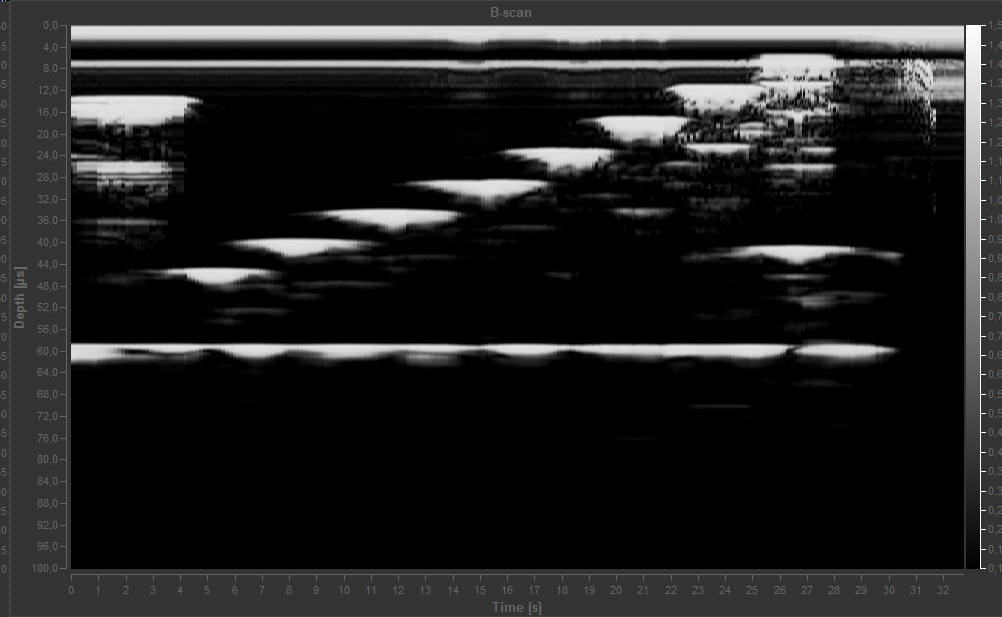
\includegraphics[width=\linewidth-40pt,height=\textheight-40pt,keepaspectratio]{content/images/B-Scan-oben.jpg}
	\label{fig:B-Scan-oben}
\end{figure}

\begin{figure}
	\centering
	\caption{B-Scan von unten}
	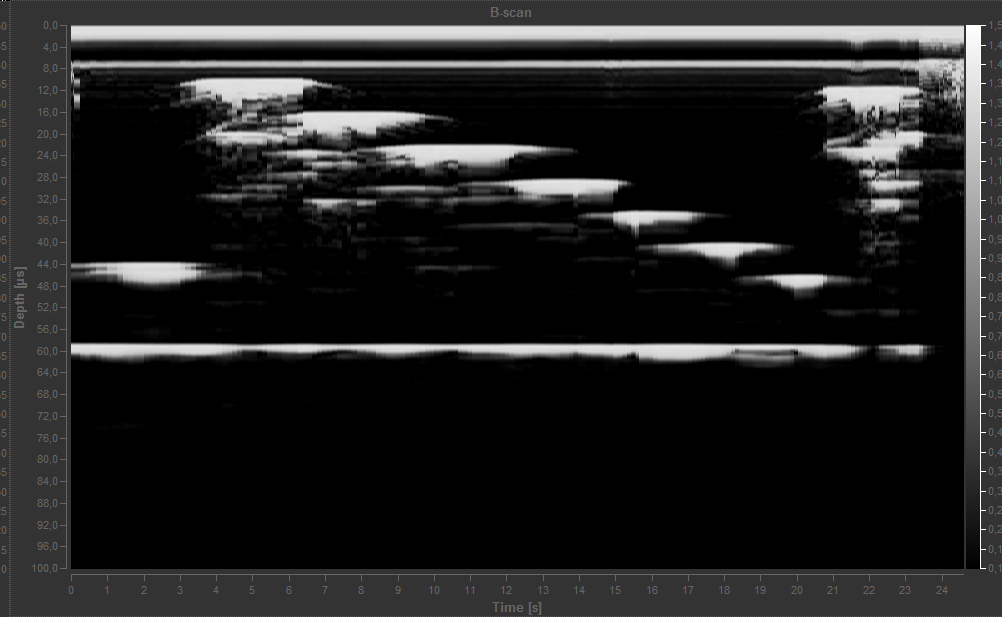
\includegraphics[width=\linewidth-40pt,height=\textheight-40pt,keepaspectratio]{content/images/B-Scan-unten.jpg}
	\label{fig:B-Scan-unten}
\end{figure}

\subsection{TM-Scan}

\begin{table}
	\centering
	\caption{B-Scan Messung}
	\label{tab:tabTMScan}
	\sisetup{table-format=1.2}
	\begin{tabular}{S[table-format=1.0]S[table-format=1.2]S[table-format=2.2]S[table-format=2.2]}
		\toprule
		{$n$} & {$\Delta t_.{n\rightarrow n+1}/\si{\second}$} &{$\Delta t_.{h}/10^{-6}\si{\second}$} & {$h/10^{-3}\si{\metre}$} \\
		\midrule
		1 & 2.28 & 30.98 & 23.00 \\
		2 & 2.03 & 32.74 & 24.31 \\
		3 & 2.03 & 31.18 & 23.15 \\
		4 & 2.03 & 32.16 & 23.88 \\
		5 & 1.97 & 32.16 & 23.88 \\
		6 & 1.91 & 33.32 & 24.74 \\
		7 & 1.91 & 33.32 & 24.74 \\
		8 & 1.73 & 31.56 & 23.43 \\
		9 & 1.79 & 32.16 & 23.88 \\
		10 & 1.85 & 32.16 & 23.88 \\
		11 & 1.66 & 30.60 & 22.72 \\
		12 & 1.79 & 30.98 & 23.00 \\
		13 & 1.73 & 31.76 & 23.58 \\
		14 & 1.79 & 31.96 & 23.73 \\
		15 & 1.73 & 31.76 & 23.58 \\
		16 & 1.60 & 30.98 & 23.00 \\
		17 & 1.66 & 30.78 & 22.85 \\
		18 & 1.73 & 31.76 & 23.58 \\
		19 & 1.60 & 32.34 & 24.01 \\
		20 & 1.60 & 32.34 & 24.01 \\
		21 & 1.60 & 33.12 & 24.59 \\
		22 & 1.66 & 30.98 & 23.00 \\
		23 & 1.60 & 31.56 & 23.43 \\
		24 & 1.60 & 30.00 & 22.28 \\
		25 & nan & 30.00 & 22.28 \\
		\bottomrule
	\end{tabular}

	\label{tab:TMScan}
\end{table}

\begin{figure}
	\centering
	\caption{TM-Scan}
	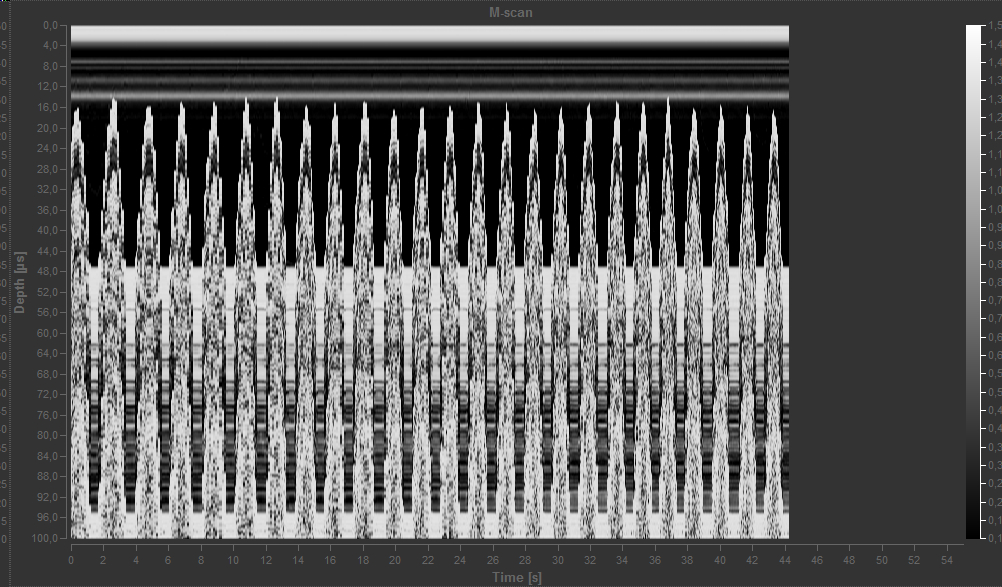
\includegraphics[width=\linewidth-40pt,height=\textheight-40pt,keepaspectratio]{content/images/TM-Scan.jpg}
	\label{fig:TM-Scan}
\end{figure}